\section{Extraction des paramètres}

Une fois la qualité des mesures évaluée, il s'agit maintenant d'en extraire les paramètres nécessaires à la fois à la synthèse par FRF et à la synthèse modale.

\subsection{Paramètres de synthèse FRF}

Dans le cadre de la première, l'admittance $Y_{body}$ du corps sans corde de l'instrument est obtenue de façon directe au travers des mesures de la partie précédente : ne restent à être extraites uniquement les valeurs des fréquences de résonance de la corde et celles de leurs amortissements.\\

Pour ce faire, et en se basant sur la relation \ref{eq:eq_frf_1}, il est en théorie possible de commencer par extraire $Y_{string}$ des valeurs mesurées de $Y_{body}$ et $Y_{total}$ puis d'analyser $Y_{string}$ et d'identifier au moyen de la relation \ref{eq:eq_frf_4} les fréquences et amortissements. Malheureusement il existe entre l'admittance de corde et les deux autres une différence d'ordre de grandeur telle que les simple bruit de mesure de ces dernières noie le signal qui aurait du être $Y_{string}$ : cela nous pousse donc à la mesurer directement sur banc de corde, ce qui par manque de temps ne sera pas fait au cours de ce projet. La suite de cette partie s'attache cependant à mettre en place un protocole d'extraction des fréquences et amortissement en supposant la connaissance de $Y_{string}$.\\

\subsubsection{Analyse ESPRIT par bandes}
\label{esprit}

Supposons donc que nous disposions d'une admittance $Y$, issue d'une mesure sur corde : il est donc à priori possible, en extrayant sa fréquence fondamentale via produit spectral, puis en recherchant chaque harmonique sur une plage de fréquence dictée par les valeurs des harmoniques précédents, d'obtenir une première série de valeurs de fréquences de modes. Cette méthode n'a cependant pas le mérite d'être très précise, et ne renvoie pas non plus de valeurs d'amortissement : elle peut cependant servir de base à une analyse par méthode à haute-résolution (dans le cas présent, la méthode ESPRIT~\cite{badeau2005methodes}) centrée autour de ces premières approximations de fréquences.\\
Le signal est dans un premier temps filtré autour de chacun de ces harmoniques par filtre passe-bande à réponse finie et phase linéaire, ceci afin de garantir des signaux filtrés présentant les mêmes pôles que le signal d'origine (le résultat est visible en~\ref{pre_proc} (b)). Afin d'accélérer l'analyse par méthode ESPRIT, il est ensuite modulé par la fréquences de l'harmonique approximatif afin de la recentrer autour de $\si{0\Hz}$ (voir~\ref{pre_proc} (c)) et de permettre une décimation (voir~\ref{pre_proc} (d)). S'ensuit alors une analyse par ESPRIT, qui donne directement accès aux valeurs exactes de fréquences propres et amortissement de $Y$.

\begin{figure}[hpbt]
\centering
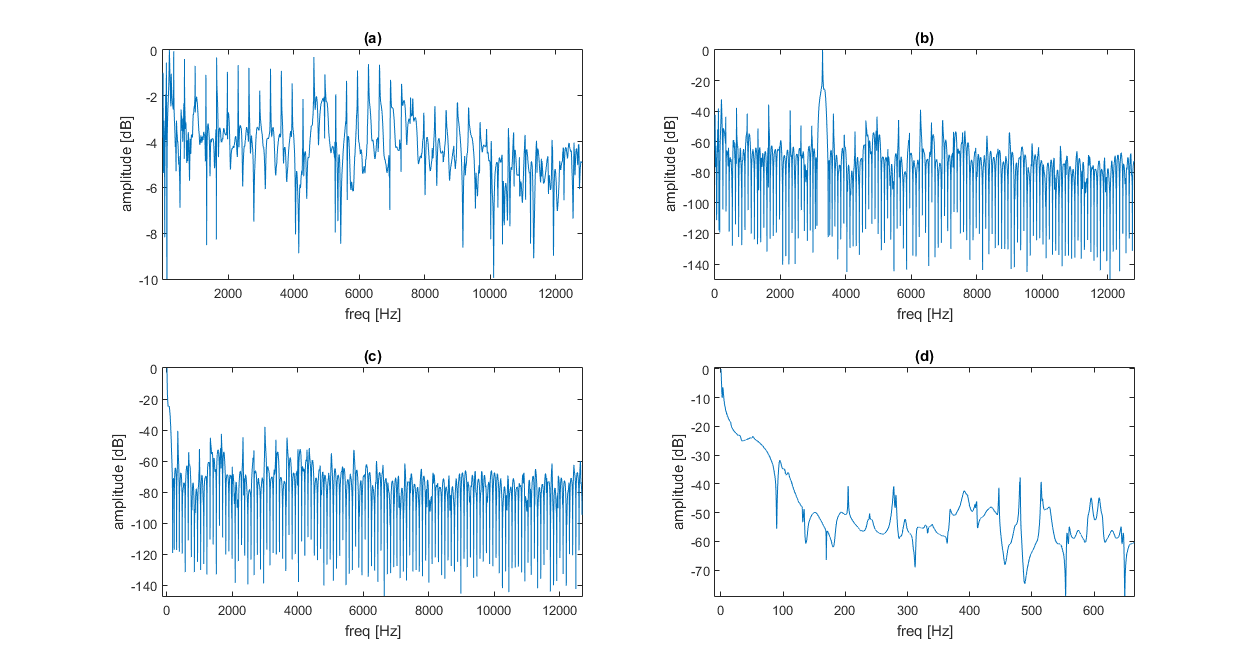
\includegraphics[width=\linewidth]{figures/pre_proc.png}
\caption{\textit{(a)~Spectre du signal d'entrée, (b)~Spectre du signal filtré sur une harmonique, (c)~Spectre du signal modulé par la fréquence de l'harmonique,
(d)~Spectre du signal décimé}}
\label{pre_proc}
\end{figure}

\subsubsection{Valeurs utilisées}

A défaut d'utiliser ce protocole pour extraire les paramètres de la synthèse par FRF, les valeurs fournies par~\textcite{woodhouse2004plucked} seront utilisées.

\subsection{Paramètres de synthèse modale}

Les paramètres utilisés en entré de la synthèse modale sont des paramètres physiques, notamment :
\begin{itemize}
 \item Tension \( T \), raideur de flexion \( B \), longueur \( L \) et
  masse linéique \( \rho \) pour la corde,
 \item Facteurs de qualité pour les modes de corde et de corps en isolation,
 \item Admittance de corps pour calculer les masses effectives,
 \item Fréquences propres et amortissements pour les modes de corps.
\end{itemize}
N'ayant pu les mesurer pour la plupart, nous utiliserons des valeurs pour
partie fournies par Woodhouse dans son article de mesures,
% (\( T, B, L, \rho \)),
% pour partie calculées par des modèles théoriques
% proposés par Woodhouse (facteurs de qualité de la corde)
ou des valeurs mesurées.
\\\\

Les paramètres ayant été rassemblés, il est maintenant possible de produire par chacune des méthodes de synthèses un son dont les conditions initiales sont contrôlées.

\section{Analyse des résultats}
Afin de pouvoir comparer les résultats de synthèse à un signal réel obtenu par mesure, nous utilisons $y_{string,wire}$ comme référant et implémentons ses conditions initiales (à savoir une impulsion de force à une distance donnée du chevalet) dans nos deux algorithme de synthèse.\\
Afin de comparer les signaux de synthèse au signal mesuré, il est entièrement possible d'utiliser le protocole développé en partie \ref{esprit} afin d'extraire les paramètres de de signaux de corde et qui renvoyait les valeurs des fréquences de résonances et leurs atténuation.\\

\begin{figure}[hpbt]
\centering
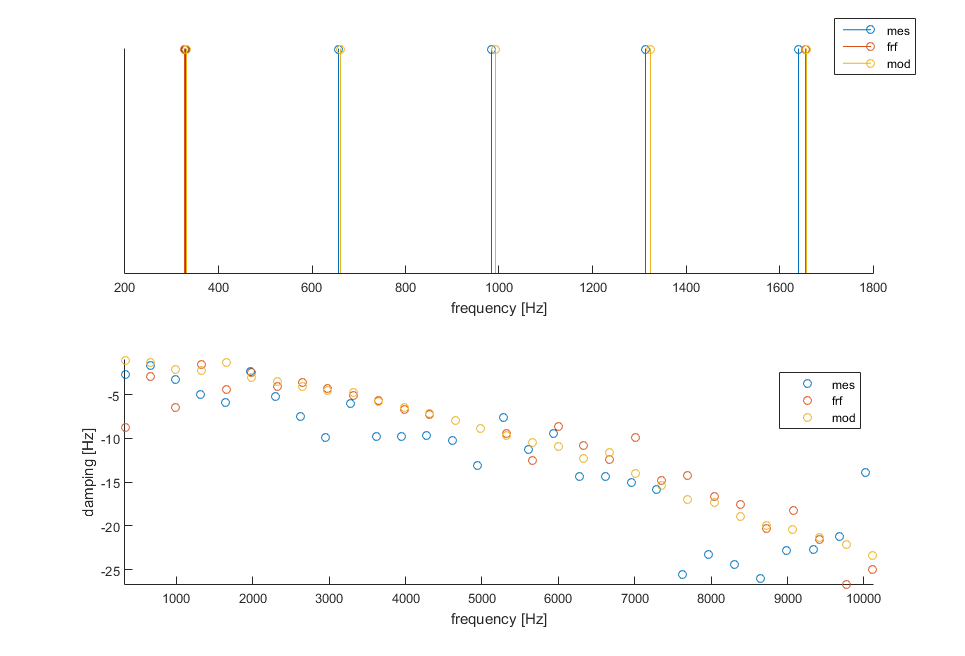
\includegraphics[width=\linewidth]{figures/apotheose.png}
\caption{En haut : fréquences de résonances des différents signaux (synthèses et réel), en~bas : atténuations en fonction des fréquences de résonance%
\label{fig:apo}}
\end{figure}

Les résultats de ces extractions de paramètres sont visibles en figure~\ref{fig:apo}. Les fréquences des deux méthodes de synthèses restent identiques, même en haute-fréquences, mais différent peu à peu de la fréquence du signal réel : cela peut être compris comme étant due à l'inharmonicité intrinsèque de la corde réelle qui, au contraire de celle issue du couplage avec le corps, n'est pas prise en compte par nos modèles de corde. Les atténuations sont satisfaisantes, puisqu'elles décrivent la même allure décroissante que celle du signal réel.

